\chapter{Mobile Application: English Mind}
\label{chap:mobile-application-english-mind}

English Mind is a mobile application available on Android \cite{cite:english_mind_play_store} and iOS \cite{cite:english_mind_app_store} platforms that focuses on learning English vocabulary. To achieve high efficiency in learning new English vocabulary, the application combines three main teaching methods on which it is based \cite{cite:english_mind_website}:

\begin{itemize}
    \item Frequency list of English vocabulary
    \item Active recall utilizing flashcards
    \item Spaced repetition system
\end{itemize}

These methods create a structured and efficient approach to mastering vocabulary with minimal effort, setting the app apart from its competitors in the field of vocabulary learning apps.

\section{Frequency List}

Frequency list is a ranked list of words, where individual words are ordered according to their frequency of occurrence in common texts and speech. 

One possible use of frequency lists is in the area of vocabulary teaching for foreign language learners. If the student learns new vocabulary words sequentially according to a frequency list, the student will encounter the newly learned words more often outside of the learning environment and thus understand more of the foreign text and speech. Conversely, if the student were to learn vocabulary randomly, the student is more likely to learn vocabulary that is too difficult relative to his current language skills, which would reduce the effectiveness of the learning process and slow his or her progress.

The importance of teaching English vocabulary according to the frequency list is supported by the results of the study \textit{How Large a Vocabulary is Needed For Reading and Listening?} \cite{cite:nation2006_how_large_vocabulary_is_needed}. This looked at how much word-family vocabulary is needed to understand most written English text and speech. The results showed that a 1,000 word-family vocabulary is needed to understand 78-81\% of most written text and a 8,000-9,000 word-family vocabulary is needed to understand 98\% of most written text. These data show the important role that frequency lists represent in effective vocabulary acquisition. If a student learns new vocabulary according to a frequency word list, he or she will understand more of the text and conversations much sooner than if he or she learns new vocabulary randomly.

\subsection*{Implementation in English Mind}

The specific implementation of the English vocabulary frequency list in the mobile application is as follows. All the vocabulary words are sorted in the app according to their frequency of occurrence in common speech and English texts. As shown in Figure~\ref{fig:em-frequency-list}, user has the possibility to browse through the ranked words and change their status. 

\begin{figure}[!h]
    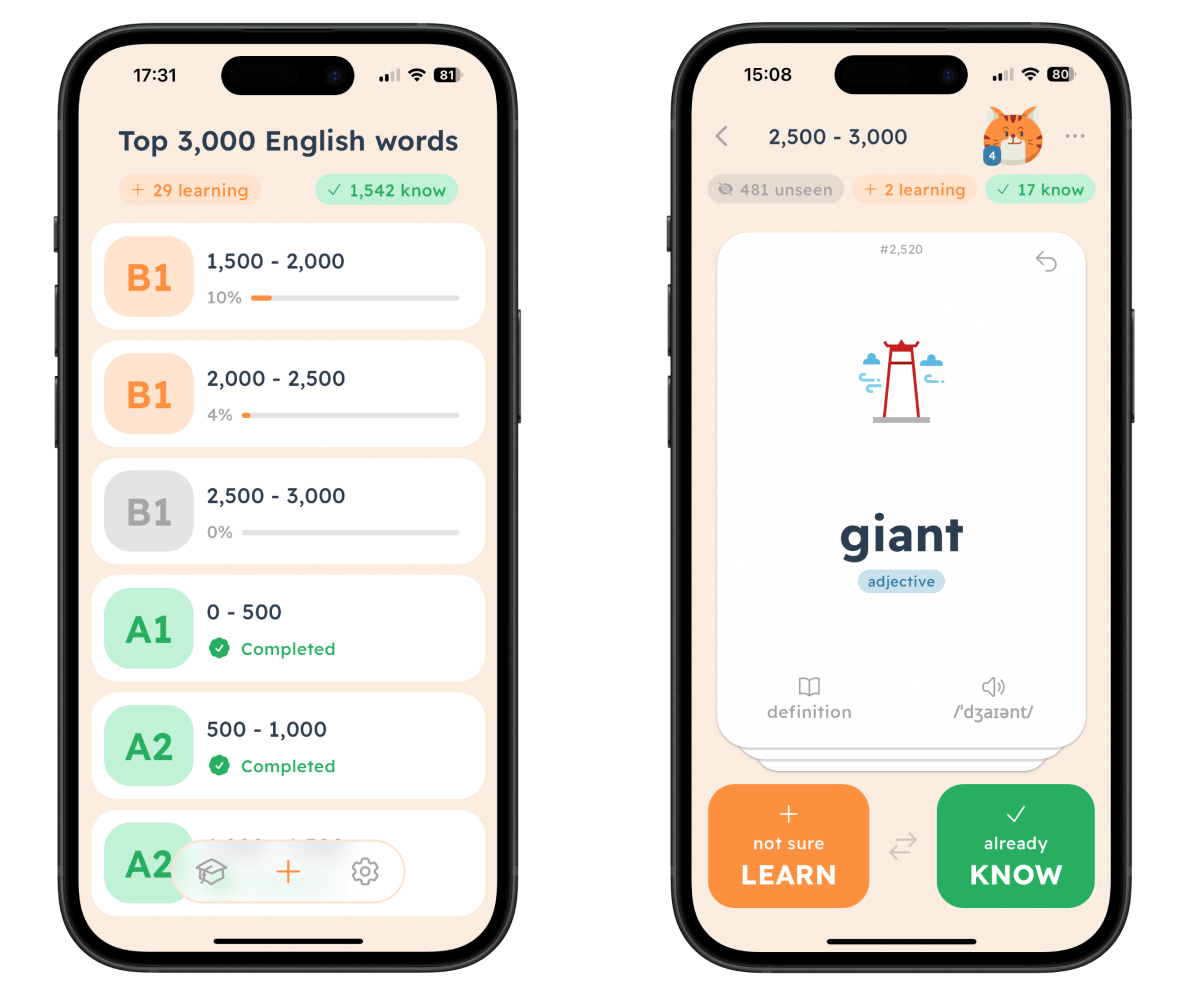
\includegraphics[width=0.65\textwidth]{src/figures/em-frequency-list.png}
    \caption{English Mind - Implementation of a Frequency List}
    \label{fig:em-frequency-list}
\end{figure}

Each word has a status that can take three different values - unseen, know or learning. The default status value is unseen, which represents words that the user has not yet encountered in the application and has not expressed whether or not he knows the word. Words with the know status represent words that the user considers to be familiar to him and does not need to practice them. The learning status, on the other hand, represents words that the user does not know and would like to learn. These learning status vocabulary words are then practiced by the user using flashcards and the spaced repetition system method, which are discussed in later chapters.

\section{Active Recall and Flashcards}

Active recall is a method that focuses on how information is repeated during learning. The aim of the method is for the student to actively try to recall the correct answer instead of memorizing the information by rereading the correct answer (passive review). Both methods, active recall and passive review, have advantages and disadvantages. However, in the area of effective vocabulary learning, active recall seems to be preferable as it achieves better results for long-term memorization of information (in our case, vocabulary words).

This is shown in a study conducted at Washington University in 2006 \cite{cite:rhkj2006_longterm_retention}, which involved reading a text and then testing its comprehension. The text for reading comprehension was divided into 30 idea units for scoring purposes. A total of 120 students between the ages of 18 and 24 participated in the study and were divided into three groups. The groups differed in the amount of time (5 minutes, 2 days, 1 week) between reading the text and taking the assessment test. Each of the three groups was further divided into two subgroups, with the first subgroup having twice as much time to memorize and understand the text. The second subgroup had only one half of the time to read the text, but compared to the first subgroup, they had the opportunity to use the active recall method in the other half of the remaining time. The final results of the study showed that the active recall method appears to be more successful for remembering information for a longer time interval compared to the passive review method (see Figure \ref{fig:active-recall-passive-review-results}).

\begin{figure}[!h]
    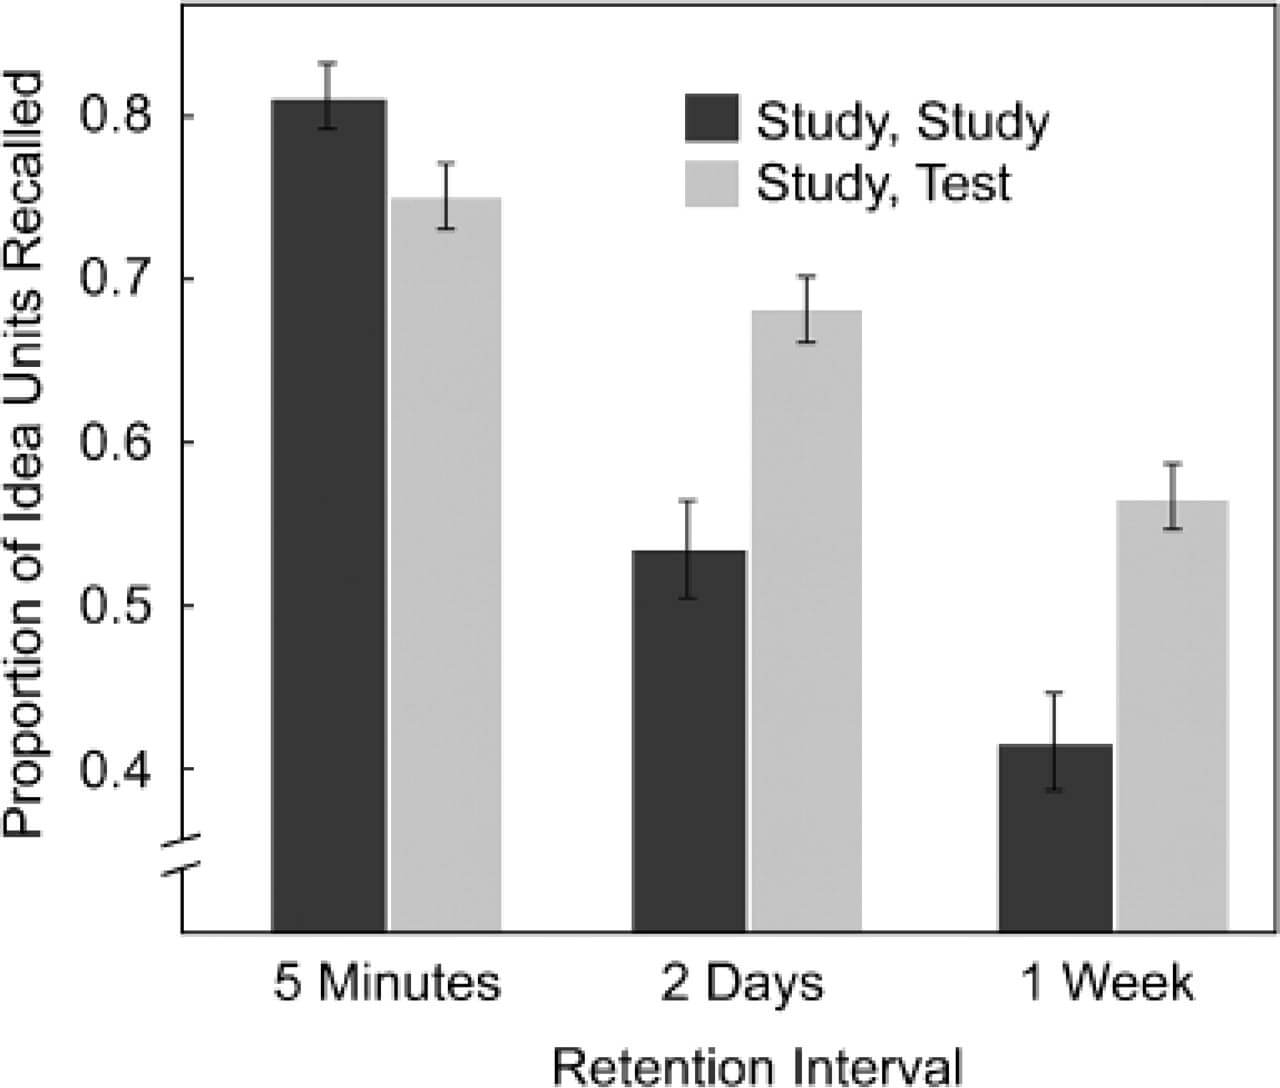
\includegraphics[width=0.6\textwidth]{src/figures/active-recall-passive-review-results.jpeg}
    \caption{Mean proportion of idea units recalled on the final test after a 5-min, 2-day, or 1-week retention interval as a function of learning condition (passive review vs. active recall). Error bars represent standard errors of the means. \cite{cite:rhkj2006_longterm_retention}}
    \label{fig:active-recall-passive-review-results}
\end{figure}

One of the most common implementations of the active recall method is using flashcards. The principle of flashcards is based on paper cards where the student writes a question on one side and the answer on the other side. While learning, the student goes through the flashcards by first asking the question without seeing the correct answer, and after answering the question, he can immediately check the correctness of his answer by flipping the flashcard over. This gives him immediate feedback and he can easily see which questions he already knows and which he needs to repeat.

\subsection*{Implementation in English Mind} 
\label{sec:em-active-recall-flashcards}

The mobile application implements the active recall method using the flashcards mentioned above. On the front side of the flashcard there is an English word and on the other side the meaning of the word in the form of a definition, sample sentences for better understanding of the use of the word, pronunciation, picture and translation into the user's native language (see Figure \ref{fig:em-flashcards}). The user goes through the flashcards one by one and always tries to actively recall the meaning of the vocabulary and its usage before revealing the second side of the flashcard. 

\begin{figure}[!h]
    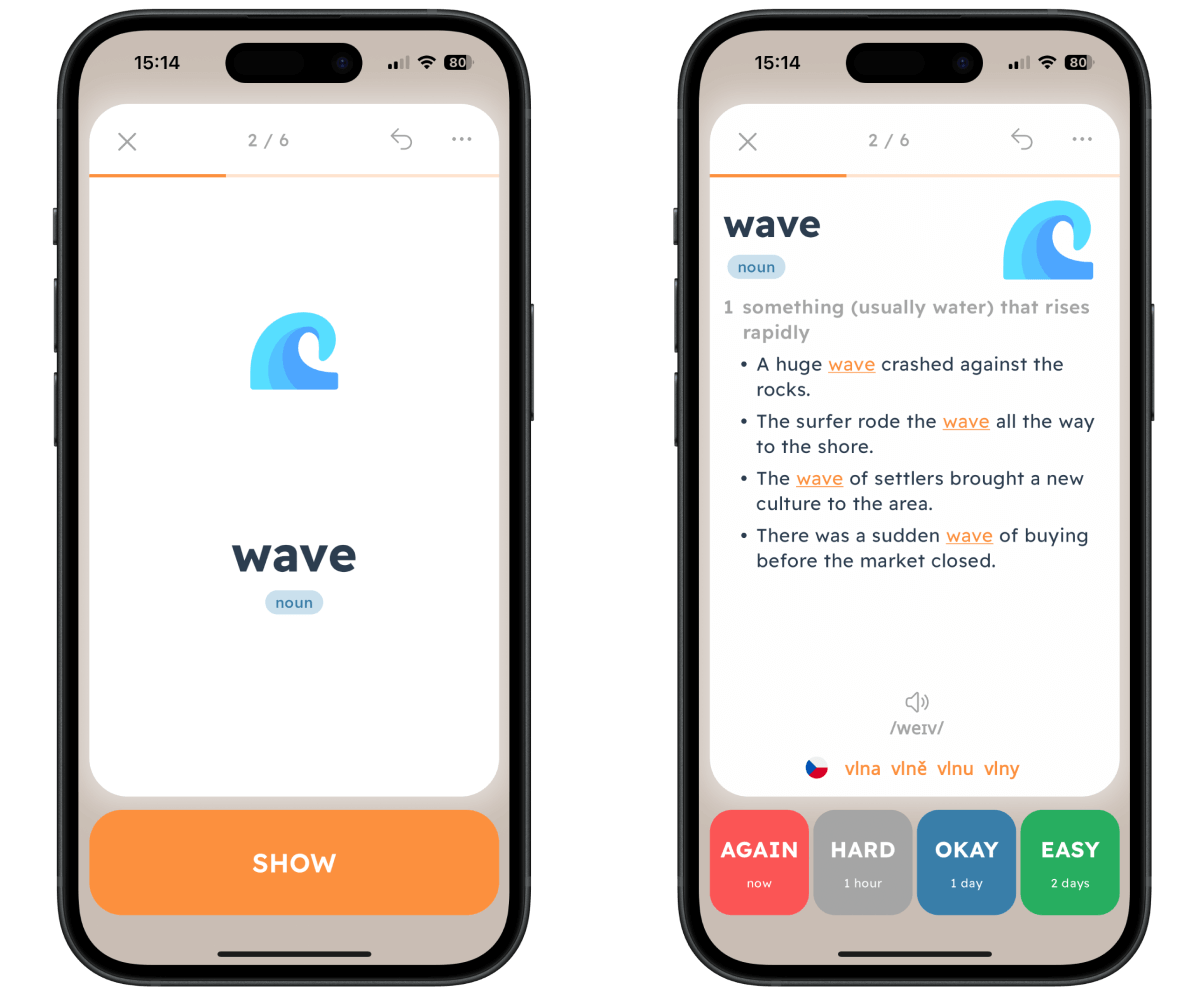
\includegraphics[width=0.65\textwidth]{src/figures/em-flashcards.png}
    \caption{English Mind - Implementation of Active Recall Utilizing Flashcards}
    \label{fig:em-flashcards}
\end{figure}

\section{Spaced Repetition System (SRS)}

The Spaced Repetition System (SRS) is a teaching method that uses time intervals between repetitions to improve long-term retention of information. The principle of SRS is based on the theory of forgetting first formulated by German psychologist Hermann Ebbinghaus in the 19th century \cite{cite:ebbinghaus2013_memory_contribution_to_experimantal_psychology}. He found out that we forget most of the information shortly after learning it, but if the information is repeated just before we begin to forget it, it can be retained much longer.

A key aspect of SRS is adjusting the length of the intervals between repetitions based on how well the student remembers the information. Information that is easily remembered by the student is repeated less often, while information that is forgotten more quickly is repeated more often \cite{cite:kang2016_spaced_repetiton_promotes_efficient_learning}.

SRS greatly increases learning efficiency and promotes long-term retention of information by optimizing the timing of repetition based on the forgetting curve, minimizing the time spent unnecessarily repeating already well-remembered information \cite{cite:kang2016_spaced_repetiton_promotes_efficient_learning}.

\subsection*{Implementation in English Mind}

Spaced repetition system is implemented in the application as follows. The user adds a word he wants to learn by changing its status to learning. The word is then displayed to the user in a queue of flashcards to practice. As the user goes through the flashcards queue, the second side of the flashcard always reveals the meaning of the vocabulary word with four SRS buttons — AGAIN, HARD, OKAY and EASY (see Figure \ref{fig:em-srs-flashcard}).

\begin{figure}[!h]
    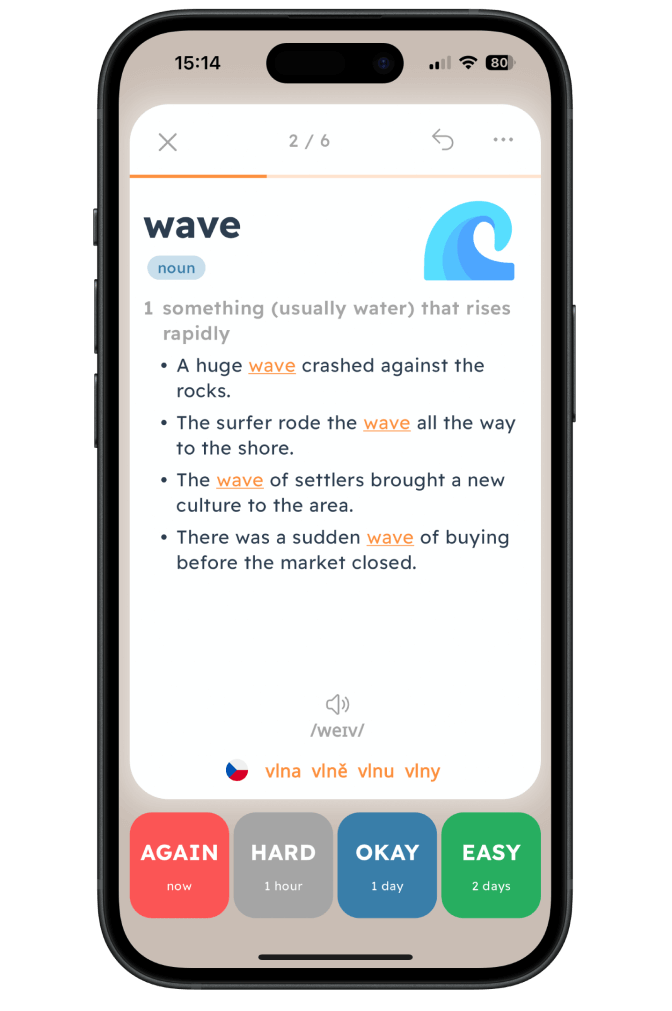
\includegraphics[width=0.42\textwidth]{src/figures/em-srs-flashcard.png}
    \caption{English Mind - Implementation of SRS (highlighted in red)}
    \label{fig:em-srs-flashcard}
\end{figure}

Each SRS button displays information about the interval between next repeating. The AGAIN and HARD buttons shorten the interval between the next repetition, while the OKAY and EASY buttons lengthen the interval. When the selected interval has elapsed, the word will appear again in the flashcards queue for practice.

When a certain interval of several months between repetitions is reached, the vocabulary is considered to have been learned. This vocabulary will automatically change its status from learning to know and will no longer appear in the user's vocabulary queue.
